\section{theory}\label{sec:theory}
In this section we will present the main contribution of the paper:
First we present the abstract syntax of the programs that the analysis is defined for, further we define the conversion from program to program graph and give the abstract syntax for instructions appearing on the edges within such graphs.
Next we formalize the abstract semantics, and thereafter we argue, through several proof sketches, that the abstract semantics are sound.
At last we prove that our analysis will always terminate.

\subsection{Abstract Syntax} \label{subsec:function-definitions}
% Casper says: The reader should know what abstract syntax is...
% This section will introduce the syntactic sets and abstract syntax of SQAAL.
% The syntactic sets of SQAAL encompass the various elements and constructs that constitute the language's grammar.
% These sets define the valid combinations of symbols and keywords that form syntactically correct statements in SQAAL. They include components such as keywords, identifiers, operators, literals, and punctuation marks, each serving a specific role in expressing queries and analytical operations.

This paper adopts a modified version of the abstract syntax originally presented in~\cite{cortesi_abstract_2013}.
Omitted parts within this simplified abstract syntax correspond to features or constructs that are not utilized or discussed in the context of the current application.
Certain constructs have been modified to enhance clarity, most notably:
\begin{itemize}
    \item variables representing database names $v_d \in \mathbb{V}_d$ has been introduced.
    \item Database variables from~\cite{halder_abstract_2012} are now called column variables, in symbols $v_t \in \mathbb{V}_t$.
\end{itemize}

The abstract syntax of SQAAL is defined in terms of the syntactic sets introduced in \autoref{fig:syntatic-sets}.
\begin{figure}[htb!]
     \center
    \begin{tabular}{r p{0.6\columnwidth }}
    $n \in \mathbb{Z}$                          & Integers                                                   \\
    $k \in \mathbb{S}$                                  & Strings                                                    \\
    $c \in \mathbb{C}$                          & Constants                                                 \\
    $v_a \in \mathbb{V}_a$                      & Application variables                                     \\
    $v_d \in \mathbb{V}_d$                      & Database variables \\
    $v_t \in \mathbb{V}_t$                    & Column variables   \\
    $v \in \mathbb{V} = \mathbb{V}_a \cup \mathbb{V}_t$ & Variables                                                 \\
    $e \in \mathbb{E}$                          & Arithmetic expressions                                    \\
    $b \in \mathbb{B}$                          & Boolean expressions                                       \\
    $\tau \in \mathbb{T}$                       & Terms                                                     \\
    $a_f \in \mathbb{A}_f$                      & Atomic formulas                                           \\
    $\phi  \in \mathbb{W}$                      & Well-formed formulas (pre-condition part of SQL commands) \\
    $A_{sql} \in \mathbb{A}_{sql}$              & Action part of SQL commands                               \\
    $C_{sql} \in \mathbb{C}_{sql}$              & SQL commands                                              \\
    $I \in \mathbb{I}$                          & Instructions/commands                                     \\
    \end{tabular}
    \caption{Syntatic Sets}
    \label{fig:syntatic-sets}
\end{figure}

The abstract syntax of SQAAL is presented in \autoref{fig:abstract-syntax}.
For simplicity's sake we assume that $\mathbb{V}_a$, $\mathbb{V}_d$ and $\mathbb{V}_t$ are mutually disjoint.

\begin{figure}[htb!]
    \center
    \begin{tabular}{r p{0.65\columnwidth}}
        $c \Coloneqq$ & $n \mid k \mid R \mid \mathscr{I}$ \\
        $v \Coloneqq$ & $v_t \mid v_a$ \\
        $e \Coloneqq$ & $c \mid v \mid op_u\; e \mid \;e_1 op_b\; e_2$ for $op_u = \{-, lower, upper, bit\_length length\}$ and $op_b = \{+, -, *, /, ||\}$ \\

        $b \Coloneqq$ & $e_1 = e_2 \mid e_1 \leq e_2 \mid e_1 < e_2 \mid \neg b \mid b_1 \lor b_2 \mid b_1 \land b_2 \mid \texttt{true} \mid \texttt{false}$ \\

        $a_f \Coloneqq$ & $e_1 = e_2 \mid e_1 \leq e_2 \mid e_1 < e_2$ \\
        $\phi \Coloneqq$ & $a_f \mid \neg \phi_1 \mid \phi_1 \lor \phi_2 \mid \phi_1 \land \phi_2 \mid \forall v_n \phi \mid \exists v_n \phi$ \\
        $A_{sql} \Coloneqq$ & $select(v_a, v_d, \mathbf{v}_t) \mid update(v_d, \mathbf{v}_t, \mathbf{e}) \mid delete(v_d) \mid insert(v_d, \mathbf{v}_t, \mathbf{e})$ \\
        $C_{sql} \Coloneqq$ & $\langle A_{sql}, \phi \rangle $ \\
        $I \Coloneqq$ & $skip \mid v_a \coloneqq e \mid C_{sql} \mid b$ \\
    \end{tabular}
    \caption{Abstract Syntax}
    \label{fig:abstract-syntax}
\end{figure}

\subsection{Abstract Domains}\label{subsec:abstract-domains}
In the following section we will describe the abstract domains of our analysis.

\subsubsection{Abstract strings as regular expressions}\label{subsubsec:abstract_domains_strings}
We have chosen regular expressions/languages to represent the abstract domain of the family of SQL string data types.
Regular expressions/languages are used instead of more powerful representations because of the decidable nature of inclusion and equality between regular languages.

Let $\regexs$ denote the set of regular expressions; for elements of $\regex \in \regexs$, we denote the language of $\regex$ as $\lang(\regex)$.
In general, we will not distinguish between $R$ and $\lang(\regex)$ when it simplifies matters.

The lattice of $(\regexs, \subseteq, \cup, \cap)$ is a lattice but not a finite one; this is a problem: Essentially, we want the state-space of our analysis to be finite, such that we can employ the Kleene fixed-point theorem (see \autoref{thm:kleene_finite}) to prove the termination of our analysis.
If the state space is built from infinite parts, the state space itself will be infinite.
We will correct this problem later in \autoref{subsubsec:cover-lattice}.

\subsubsection{Abstract integers as union intervals}\label{subsubsec:abstract_domains_numbers}
We have chosen a finite union and intersection of intervals to represent the abstract domain of the family of SQL number data types.
We limit ourselves to finite union and intersection to ensure that operations such as inclusion and membership checking remain tractable.

We call them union intervals, as all such objects can be written as a union of intervals.
We only consider integers, but we imagine the domain can be easily extended to the reals.

Let $\mathbf{INT}$ be the set of union intervals, with members denoted $\mathscr{I}$, that is inductively defined as:


\begin{gather*}
    \inference{i \text{ is an interval}}{i \in \mathbf{INT}} \quad
    \inference{\mathscr{I}_1 \in \textbf{INT} \quad \mathscr{I}_2 \in \textbf{INT}}{\mathscr{I}_1 \cup  \mathscr{I}_2 \in \mathbf{INT}}\\
    \inference{\mathscr{I}_1 \in \textbf{INT} \quad \mathscr{I}_2 \in \textbf{INT}}{\mathscr{I}_1 \cap  \mathscr{I}_2 \in \mathbf{INT}}
\end{gather*}


For the set of integers $\mathbb{Z}$, we will only consider $\emptyset, [a, b], [a, +\infty]$ and $[-\infty, b]$ where $a \leq b$ and $a, b \in \mathbb{Z}$, as valid intervals.

We define the language of union intervals as follows:


\begin{align*}
    \lang(\uint_1 \cup \uint_2) &= \lang(\uint_1) \cup \lang(\uint_2) \\
    \lang(\uint_1 \cap \uint_2) &= \lang(\uint_1) \cap \lang(\uint_2) \\
    \lang(\emptyset) &= \emptyset \\
    \lang([a, b]) &= \left\{ n \in \nums \middle| a \leq n \leq b \right\} \\
    \lang([a, +\infty]) &= \left\{ n \in \nums \middle| a \leq n \right\} \\
    \lang([-\infty, b]) &= \left\{ n \in \nums \middle| n \leq b \right\}
\end{align*}


Similarly to the abstract domain of strings, we generally don't distinguish between a union interval $\uint$ and its language $\mathcal{L}(\uint)$ when it simplifies matters.
Furthermore, this abstract representation of numbers $(\uints, \subseteq, \cup, \cap)$ has the same issue as regular expressions: It is not finite.

This abstract domain is most likely not a new development, the title of~\cite{li2010abstract} suggest a similar construct, but we have been unable to get a hold of their paper.

\subsubsection{Cover lattices}\label{subsubsec:cover-lattice}
To resolve the issue of non-finite lattices presented above, we introduce the notion of a cover lattice.
As mentioned above, the idea presented here is probably not novel.

Before we can define a cover lattice, we need to define the notion of a top-cover.

\begin{definition}
    A finite non-empty subset $X \subseteq S$ of a lattice $(S, \subseteq, \cup, \cap)$ is called a top-cover of $S$ whenever $\bigcup X = \top$.
\end{definition}

\begin{definition}\label{def:coverlattice}
Given a top-cover $X$ of a lattice $(S, \subseteq, \cup, \cap)$.
A cover lattice of $S$ in respect to $X$ denoted $\clattice{X}{S}$ is the set inductively defined as:

\begin{gather*}
    \inference{x \in X}{x \in C_X(S)} \quad
    \inference{x_1 \in C_X(S) \quad x_2 \in C_X(S)}{x_1 \cup  x_2 \in C_X(S)}\\
    \inference{x_1 \in C_X(S) \quad x_2 \in C_X(S)}{x_1 \cap  x_2 \in C_X(S)}
\end{gather*}
\end{definition}

As a note when we use the notation $C_X(S)$ we always assume that $X$ is a top-cover of $S$.
The notion of a cover lattice gives rise to the following theorem:

\begin{restatable}{theorem}{partition}\label{thm:partition}
For a non-complete lattice $(S, \subseteq, \cup, \cap)$ and top-cover $X$ of $S$, the cover lattice $(\clattice{X}{S}, \subseteq, \cup, \cap)$ is a finite and complete lattice.
\end{restatable}

And the following corollaries immediately follow:

\begin{corollary}\label{co:topcoverr}
    If $\mathcal{R}$ is a top-cover of $(\regexs, \subseteq, \cup, \cap)$ then $(\clattice{\mathcal{R}}{\regexs}, \subseteq, \cup, \cap)$ is a finite and complete lattice.
\end{corollary}

\begin{corollary}\label{co:topcoveri}
    If $\mathcal{I}$ is a top-cover of $(\uints, \subseteq, \cup, \cap)$ then $(\clattice{\mathcal{I}}{\uints}, \subseteq, \cup, \cap)$ is a finite and complete lattice.
\end{corollary}

We now define the function that maps elements in a lattice to the most precise element in a corresponding cover lattice:

\begin{align}
    \cdot \into C_X(S) &: S\rightarrow C_X(S) \\
    s \into C_X(S) &= \bigcap\{s' \in C_X(S)|s \subseteq s'\}
\end{align}

We overload this notation to work on sets of values in particular for $S' \subseteq S$ we define:

\begin{align}
    \cdot \into C_X(S) &: \mathcal{P}(S) \rightarrow \mathcal{P}(C_X(S)) \\
    S' \into C_X (S) &= \{s \into C_X(S) \mid s \in S'\}
\end{align}

To make this notion useful we assume that some mapping from application variables and table attributes to cover lattices is given by the user by some mechanism\footnote{We discuss such mechanisms in \autoref{sec:discussion}.}:

\begin{equation}\label{eq:lookupcl}
    \lookupcl : \mathbb{V} \rightarrow \{ C_{X_1}(S_1), C_{X_2}(S_2), \dots, C_{X_n}(S_n) \}
\end{equation}


Where for all $1 \leq i \leq n$ either $S_i = \regexs$ with some $X_i = \mathcal{R} \subset \regexs$ or $S_i = \uints$ with some $X_i = \mathcal{I} \subset \uints$.
Further we define the following helper function $c$, relating cover lattices to their concrete counterpart:


\begin{align}
    c(C_{\mathcal{R}}(\regexs)) &= \strs \\
    c(C_{\mathcal{I}}(\uints)) &= \nums
\end{align}


Where $\strs$ are the set of all strings and $\nums$ the set of all integers.

Now we are able to express the concretization for regular expressions and union intervals.

\begin{align}
    &\concrete^v_6 : \lookupcl(v) \rightarrow \powerset{\cc(\lookupcl(v))} \\
    &\concrete^v_6(Y) = \mathcal{L}(Y)
\end{align}

Where $Y$ is a regular expression or union interval.

% \begin{definition}
%     We define $\cdot \into C_X(S):S\rightarrow C_X(S)$ to be the function mapping $s\in S$ to the least element in $C_X(S)$ containing it, that is $s \into C_X(S)=\bigsqcap\{s'\in C_X(S)|s\sqsubseteq s'\}$
%     \\
%
%     We define $\cdot \into C_X(S):\mathcal{P}(S)\rightarrow \mathcal{P}(C_X(S))$ to be the function that maps the powerset$(\mathcal{P})$ of the lattice elements to the powerset of the cover lattice elements$(C_X (S))$.
%     We use $H \into C_X (S) = \{h \into C_X (S) \mid h \in H\}$ to show how a set of elements$(H)$ is mapped to the cover lattice.
% \end{definition}

% todo I don't think the definition below is ever used, uncomment it if you find a case
% \begin{definition}
%     We define $\cdot \into C_\mathcal{X}(\mathcal{S}): \bigtimes_{i = 1}^{n} S_i \rightarrow \bigtimes_{i = 1}^{n} C_{X_i}(S_i)$ to be the function that takes a tuple and inserts each element of the tuple correctly into its given cover lattice.
%     We use $(h_1, h_2 \dots h_n)\into C_{\mathcal{X}}(\mathcal{S})=(h_1 \into C_{X_1}(S_1), h_2\into C_{X_2}(S_2), \dots, h_n \into C_{X_n}(S_n))$, where $\mathcal{X}=(X_1, X_2, \dots, X_n)$ and $\mathcal{S}=(S_1, S_2, \dots, S_n)$ to show how a tuples elements are inserted into the cover lattice what $\mathcal{X}$ and $\mathcal{S}$ are.
% \end{definition}

\autoref{fig:tikz-reg-partition} illustrates a simple top-cover of the regular languages.
The regular language $R$ is represented by the gray circle and its complement $\overline{R}$ is represented by the white circle.
The union of the two regular languages is the universal language $\Sigma^*$.

\autoref{fig:tikz-reg-partition-lattice} illustrates the cover lattice induced by the cover-lattice.
The top element $\top$ is the entire regular language $\Sigma^*$ and the bottom element $\bot$ is the empty set $\emptyset$.


% Tikzfigures
\begin{figure}
    \center
    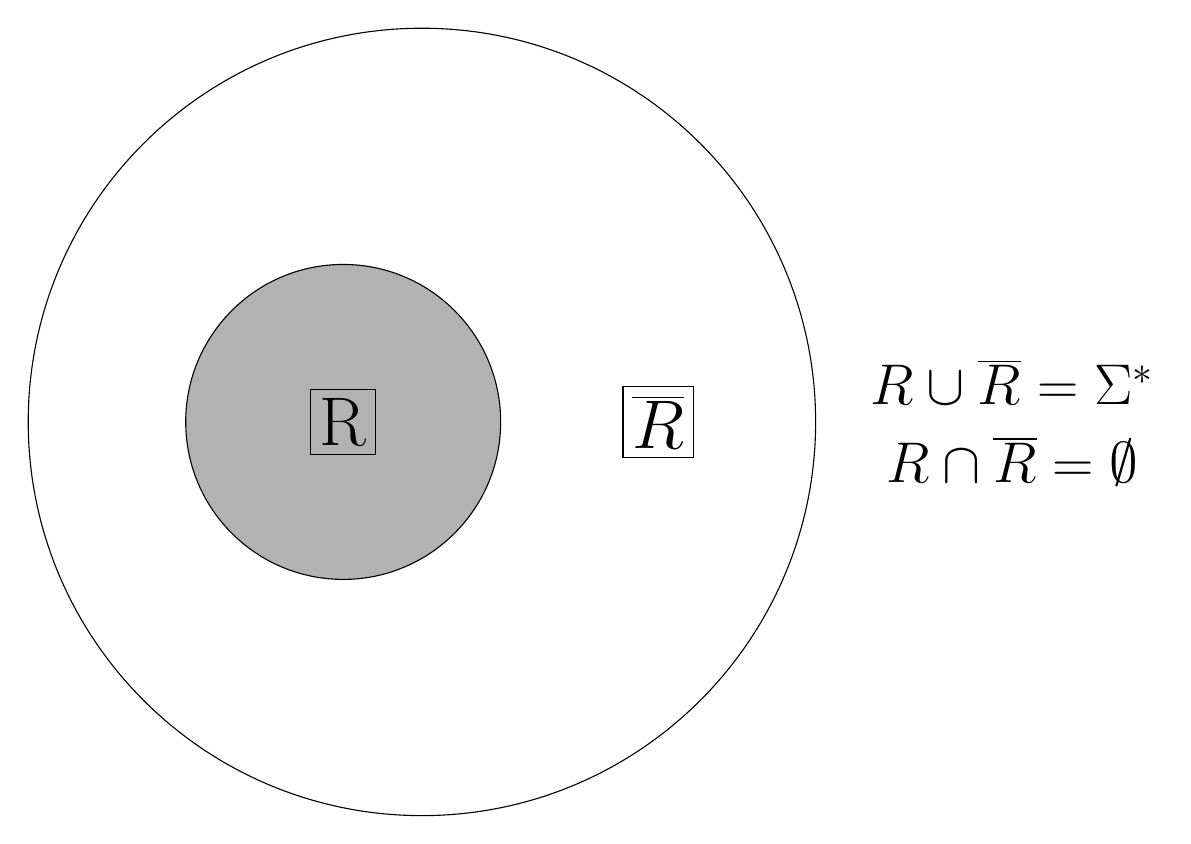
\begin{tikzpicture}
    \filldraw[fill=white, draw=black] (2,2) circle (5cm);
    \node [draw] at (5,2) {\Huge$\overline{R}$};
    \filldraw[fill=gray!60, draw=black] (1,2) circle (2cm);
    \node [draw] at (1,2) {\Huge R};
    \node at (9.5, 2.5) {\huge $R \cup \overline{R} = \Sigma^*$};
    \node at (9.5, 1.5) {\huge $R \cap \overline{R} = \emptyset$};
\end{tikzpicture}
    \caption{Regular language top-cover}
    \label{fig:tikz-reg-partition}
\end{figure}

\begin{figure}[!htb]
    \center
    \begin{tikzpicture}[scale = 0.5]
    \usetikzlibrary{calc}
    \node (a) [state] {\Huge$R \cup \overline{R} = \top = \Sigma^*$};
    \node (b1) [state, shift={($(a.south)+(3cm, -2.5cm)$)}] {\Huge $R$};
    \node (b2) [state, shift={($(a.south)+(-3cm, -2.5cm)$)}]{\Huge $\overline{R}$};
    \node (c) [state, shift= {($(a.south) + (0cm, -5.5cm)$)}] {\Huge $R \cap \overline{R} = \bot = \emptyset$};
    \draw (a) to (b1);
    \draw (a) to (b2);
    \draw (b1) to (c);
    \draw (b2) to (c);
\end{tikzpicture}
    \caption{Cover lattice induced by regular expressions}
    \label{fig:tikz-reg-partition-lattice}
\end{figure}

\subsubsection{Abstract tuples}\label{subsubsec:abstract-tuples}
We define abstract tuples as the product cover lattices of $\regexs$ and $\uints$ intertwined depending on the schema of the table.
The concretization function is defined as follows:


\begin{gather}
    \concrete^{v_1, v_2, \dots, v_n}_5 : \bigtimes_{i = 1}^{n}(\lookupcl(v_i)) \rightarrow \mathcal{P}\left(\bigtimes_{i = 1}^n \cc(\lookupcl(v_i)) \right)\\
    \begin{split}
        \concrete^{v_1, v_2, \dots, v_n}_5 & (\ab{e_1}, \ab{e_2}, \dots, \ab{e_n}) = \\
         &\concrete^{v_1}_6(\ab{e_1}) \times \concrete^{v_2}_6(\ab{e_2}) \times \dots \times \concrete^{v_n}_6(\ab{e_n})
    \end{split}
\end{gather}

Considering the schema in \autoref{lst:motivate-sql}, a possible abstract tuple could be $x = ([\texttt{A}-\texttt{Z}][\texttt{a}-\texttt{z}]^* \_ \; [\texttt{A}-\texttt{Z}][\texttt{a}-\texttt{z}]^*, [0, 100])$ where $[\texttt{A}-\texttt{Z}] = \{\texttt{A}, \texttt{B}, \dots, \texttt{Z}\}$, $[\texttt{a}-\texttt{z}] = \{\texttt{a}, \texttt{b}, \dots, \texttt{z}\}$ and $\_$ is the blank space character.
As an example $(\texttt{Casper Ståhl}, 99) \in \concrete_5^{\texttt{name},\texttt{balance}}(x)$.

\subsubsection{Abstract tables}\label{subsubsec:abstract_domain_of_tables}
We consider a concrete table $t$ as function from the domain of possible tuples in the table $\mathbf{TUP}$ to the codomain of natural numbers including $0$, $\mathbf{NAT}$:


\begin{equation}
    t : \mathbf{TUP} \rightarrow \mathbf{NAT}.\label{eq:equation-tup-nat}
\end{equation}


The function $t$ describes the number of occurrences a given tuple in a table.
We can then consider abstracting over a table $t$ by abstracting either the domain or codomain.
This gives rise to a taxonomy of abstract domains of tables shown in \autoref{tab:taxonomy_of_abstract_domain_of_tables}.
In \autoref{tab:taxonomy_of_abstract_domain_of_tables}, $\ab{\mathbf{TUP}}$ denotes an abstract domain of the set of possible tuples $\mathbf{TUP}$ (and analogous for $\mathbf{NAT}$).


\begin{table}
    \renewcommand{\arraystretch}{1.3}
    \caption{Taxonomy of Abstract Domains of Tables}
    \centering
    \begin{tabular}{c|l}
        \toprule
        Classification                  & Function                                \\ \midrule
        Bag of tuples                   & $\mathbf{TUP} \rightarrow \mathbf{NAT}$           \\
        Abstract bag of tuples          & $\mathbf{TUP} \rightarrow \ab{\mathbf{NAT}}$      \\
        Bag of abstract tuples          & $\ab{\mathbf{TUP}} \rightarrow \mathbf{NAT}$      \\
        Abstract bag of abstract tuples & $\ab{\mathbf{TUP}} \rightarrow \ab{\mathbf{NAT}}$ \\ \bottomrule
    \end{tabular}
    \label{tab:taxonomy_of_abstract_domain_of_tables}
\end{table}

One would classify the work in~\cite{halder_abstract_2012} as using bags of abstract tuples, and in this work, as previously mentioned, we will use abstract bags of abstract tuples.
In this work in particular we consider $\ab{\mathbf{TUP}}$ as given by the map $\lookupcl$, to be more precise:
If $attr(v_d) = (v_{t_1}, \dots, v_{t_n})$ then $\ab{\mathbf{TUP}} = \bigtimes_{i = 1}^n \lookupcl(v_{t_i})$, where $attr : \mathbb{V}_d \rightarrow \mathbb{V}_t^*r$ is given by the schema of the database.
The abstract codomain is given by $\ab{\mathbf{NAT}} = \{0, 0 \leq\}$.

Simplifying the above for our own sanity, we consider $\ab{t} : \ab{\mathbf{TUP}} \rightarrow \ab{\mathbf{NAT}}$ to be represented as a single set $\ab{t'}$ instead, that is $\ab{t}({e}) = 0 \iff e \notin \ab{t'}$ and  $\ab{t}({e}) = (0 \leq) \iff e \in \ab{t'}$.

Further, as the form of an abstract table is given by the schema and the mapping $\lookupcl$ the final formalization for some table with name $v_d$ is then $\ab{t} \in \mathcal{P}\left(\bigtimes_{i = 1}^{n}\lookupcl(v_{t_i})\right)$ for $attr(v_d) = (v_{t_1}, v_{t_2}, \dots, v_{t_n})$.

As the concretization of an abstract table is a bag we need to define a map from the underlying set $S$ to the set of all bags over that underlying set before we can define the concretization itself.

We denote that set $\mathcal{M}(S)$ and define it formally as:

\begin{equation}
    \mathcal{M}(S) = S \rightarrow \mathbf{NAT}\label{eq:equation-nums}
\end{equation}

Further we define the following notation for bags:
\begin{align}
    s \in t \iff 0 < t(s)
\end{align}

And thus we can define the concretization of a table, for $attr(v_d) = (v_{t_1}, v_{t_2}, \dots, v_{t_n})$:


\begin{gather}
    \concrete^{v_d}_{4d} : \mathcal{P}\left(\bigtimes_{i = 1}^{n}\lookupcl(v_i)\right) \rightarrow \mathcal{M}\left(\bigtimes_{i = 1}^n \cc(\lookupcl(v_i))\right)\\
    \begin{split}
        \concrete^{v_d}_{4d}(\ab{t}) = \biggl\{ &t \in \mathcal{M}\Bigl(\bigtimes_{i = 1}^n \cc(\lookupcl(v_i))\Bigr) \Big|\\
        &\forall e \in t : \exists \ab{e} \in \ab{t} : e \in \concrete^{attr(v_d)}_5(\ab{e}) \biggr\}
    \end{split}
\end{gather}

To solidify the relation, see that: $\rho_{\ab{d}}(v_d) = \ab{t}$ and $t \in \gamma_{4d}^{v_d}(\ab{t})$, where $\rho_{\ab{d}}$ is the abstract environment mapping table names to abstract tables as later defined in \autoref{subsubsec:absenv}.

\subsubsection{Abstract application variable values}
In the concrete semantics of instructions that may appear on edges (A draft of the concrete semantics can be found in \autoref{sec:concrete-semantics}), we allow application variables to be assigned to singleton values or single columns of values.

When an application variable is assigned to a column of values, such an assignment occurs either as a result of a select statement or when the expression part of an assignment contains a variable that maps to a column in the current environment.
Therefore, we would like to distinguish between the two cases as much as possible in abstract semantics.
Thus for some set $S$, we introduce the set $\mathsf{Val} \; S$ of column and singleton values arising from $S$.

Here, we differ from~\cite{halder_abstract_2012}; we do not impose an order on column values in the concrete or abstract semantics.
We inductively define $\mathsf{Val} \; S$ as follows:

\begin{gather*}
    \inference{s \in S}{\mathsf{Single} \; s \in \mathsf{Val} \; S} \quad
    \inference{S' \subseteq S}{\mathsf{Col} \; S' \in \mathsf{Val} \; S}
\end{gather*}


% todo this should be uncommented if we wan't to fix the galios connection.
% We define the partial order $\sqsubseteq$ of the lattice $(\mathsf{Val} \; A, \sqsubseteq, \sqcup, \sqcap)$ as follows:
% \begin{align}
%     \mathsf{List} \; S_1 &\sqsubseteq \mathsf{List} \; S_2 \iff \forall s_1 \in S_1, \; \exists s_2 \in S_2: \; s_1 \sqsubseteq s_2 \\
%     \mathsf{Single} \; s_1 &\sqsubseteq \mathsf{Single} \; s_2 \iff s_1 \sqsubseteq s_2 \\
%     \mathsf{Single} \; s &\sqsubseteq \mathsf{List} \; S \iff s \in S \\
%     \mathsf{List} \; S &\not\sqsubseteq \mathsf{Single} \; s
% \end{align}
% The join and meet $\sqcup$ and $\sqcap$ respectively is defined as follows here:
% \begin{align}
%     \mathsf{Single} \; s \sqcup \mathsf{List} \; S &= \mathsf{List} \; (S\sqcup\left\{ s \right\})\\
%     \mathsf{Single} \; s_1 \sqcup \mathsf{Single} \; s_2 &= \mathsf{Single} \; (s \sqcup s )\\
%     \mathsf{List} \; S_1 \sqcup \mathsf{List} \; S_2 &= \mathsf{List} \; (S_1 \sqcup S_2)\\
%     \mathsf{Single} \; s \sqcap \mathsf{List} \; S &= \mathsf{Single} \; s\\
%     \mathsf{List} \; S_1 \sqcap \mathsf{List} \; S_2 &= \mathsf{List} \; (S_1 \sqcap S_2)\\
%     \mathsf{Single} \; s_1 \sqcap \mathsf{Single} \; s_2 &= \mathsf{Single} \; (s_1 \sqcap s_2)\\
%     \mathsf{List} \ \emptyset \sqcap \mathsf{Single} \ s &= \ \perp
% \end{align}

It will be helpful to further overload the $\into$ operator for this type of values, therefore we define


\begin{align}
    \cdot \into C_X(S) &: \mathsf{Val} \; S \rightarrow \mathsf{Val} \; C_X(S) \\
    (\mathsf{Single} \; s) \into C_X(S) &= \mathsf{Single} \; (s \into C_X(S)) \\
    (\mathsf{Col} \; S') \into C_X(S) &= \mathsf{Col} \; (S' \into C_X\left(S\right))
\end{align}


And the following notation will also be helpful later:


\begin{align}
    s \in (\mathsf{Single} \; s') \iff s = s^\prime \\
    s \in (\mathsf{Col} \; S) \ \iff \ s \in S.
\end{align}


We define the concretization of application variable values as:


\begin{gather}
    \concrete^v_{4a} : \mathsf{Val} \; \lookupcl(v) \rightarrow \powerset{\cc(\lookupcl(v))} \cup \powerbag{\cc(\lookupcl(v))} \\
    \concrete^v_{4a}(\mathsf{Single} \; \ab{s}) = \concrete^v_6(\ab{s})
\end{gather}
\begin{multline}
    \concrete^v_{4a}(\mathsf{Col} \; \ab{S}) = \left( \bigcup_{\ab{s} \in \ab{S}} \concrete^v_6(\ab{s}) \right) \cup \\
    \left\{ t \in \powerbag{\cc(\lookupcl(v))}\middle| \forall e \in t : \exists \ab{s} \in \ab{S} : e \in \concrete^v_6(\ab{s}) \right\}
\end{multline}


For the purpose of proving soundness later we also overload $\gamma_{4a}$ as follows:


\begin{align}
    \concrete_{4a} &: \mathsf{Val} \; \regexs \rightarrow \powerset{\strs} \cup \powerbag{\strs} \\
    \concrete_{4a} &: \mathsf{Val} \; \uints \rightarrow \powerset{\nums} \cup \powerbag{\nums}
\end{align}

With the same \emph{implementation} as above, and:
\begin{align}
    \concrete_{4a} &: \mathcal{P}(\{\true, \false, \mnull\}) \rightarrow \mathcal{P}(\{\true, \false, \mnull\}) \\
    \concrete_{4a} &= \mathrm{id}
\end{align}



\subsubsection{Abstract environments}\label{subsubsec:absenv}
We define an abstract environment $\rho_{\ab{a}} \in \ab{\mathfrak{E}_a}$ mapping application variable names $v_a \in \mathbb{V}_a$ to abstract values, and $\rho_{\ab{d}} \in \ab{\mathfrak{E}_d}$ mapping table names $v_d \in \mathbb{V}_d$ to abstract tables.
Given the previously mentioned map $\lookupcl$ in \autoref{eq:lookupcl} we define:


\begin{align} \label{eq:absenva}
    \ab{\mathfrak{E}_a} &= \mathbb{V}_a \rightarrow \bigcup_{v_a \in \mathbb{V}_a} \mathsf{Val} \; \lookupcl(v_a) \\ \label{eq:absenvd}
    \ab{\mathfrak{E}_d} &= \mathbb{V}_d \rightarrow \bigcup_{v_d \in \mathbb{V}_d} \mathcal{P}\left(\bigtimes_{v_t \in attr(v_d)}\lookupcl(v_t)\right) \\
    \ab{\mathfrak{E}} &= \ab{\mathfrak{E}_a} \times \ab{\mathfrak{E}_d}
\end{align}


And the concrete counterparts:


\begin{align}
    \mathfrak{E}_a &= \mathbb{V}_a \rightharpoonup \nums \cup \powerbag{\nums} \cup \strs \cup \powerbag{\strs} \\
    \mathfrak{E}_d &= \mathbb{V}_d \rightarrow \bigcup_{v_d \in \mathbb{V}_d} \mathcal{M}\left(\bigtimes_{v_t \in attr(v_d)}\cc(\lookupcl(v_t))\right) \\
    \mathfrak{E} &= \mathfrak{E}_a \times \mathfrak{E}_d
\end{align}

Note that members of $\mathfrak{E}_a$ are partial functions.

And we define the concretization functions for environments as:


\begin{gather}
    \concrete_2 : \ab{\mathfrak{E}} \rightarrow \mathcal{P}(\mathfrak{E})\\
    \concrete_2(\rho_{\ab{d}}, \rho_{\ab{a}}) = \concrete_{3d}(\rho_{\ab{d}}) \times \concrete_{3a}(\rho_{\ab{a}})
\end{gather}


\begin{gather}
    \concrete_{3d} : \ab{\mathfrak{E}_d} \rightarrow \mathcal{P}(\mathfrak{E}_d)\\
    \concrete_{3d}(\rho_{\ab{d}}) = \biggl\{ \rho_{d} \in \mathfrak{E}_d \Big| \forall v_d \in \mathbb{V}_d : \rho_d(v_d) \in \concrete^{v_d}_{4d}(\rho_{\ab{d}}(v_d)) \biggr\}
\end{gather}


\begin{gather}
    \concrete_{3a} : \ab{\mathfrak{E}_a} \rightarrow \mathcal{P}(\mathfrak{E}_a)\\
    \concrete_{3a}(\rho_{\ab{a}}) = \biggl\{ \rho_{a} \in \mathfrak{E}_a \Big| \forall v_a \in \mathbb{V}_a : \rho_a(v_a) \in \concrete^{v_a}_{4a}(\rho_{\ab{a}}(v_a)) \biggr\}
\end{gather}


And in the same vein we define a concretization function for sets of environments as:


\begin{gather}
    \concrete_1 : \mathcal{P}(\ab{\mathfrak{E}}) \rightarrow \mathcal{P}(\mathfrak{E})\\
    \begin{split}
         \concrete_1(\ab{P})& = \\
        & \biggl\{ (\rho_{d}, \rho_{a}) \in \mathfrak{E}
        \Big| \exists (\rho_{\ab{d}}, \rho_{\ab{a}}) \in \ab{P} : (\rho_{d}, \rho_{a}) \in \concrete_2(\rho_{\ab{d}}, \rho_{\ab{a}})\biggr\}
    \end{split}
\end{gather}


\subsection{Abstract Semantics}\label{subsec:abstract-semantics}
This section will describe the abstract semantics of SQAAL.

\autoref{eq:generalBOP} through~\ref{eq:generalUOP}, show the definition of abstract operations on members of $\mathsf{Val} \; A$.
These operations are denoted by $\aop$, where $\aop$ is defined in \autoref{eq:operation} through \ref{eq:generalUOP}.
These equations provide a systematic way to perform abstract operations on values within $\mathsf{Val} \ A$.
The specific operations $\aaop$ are defined for the respective types later on.\todo{Gabriela: are they abstract? concrete? both? \\ Casper: It doesn't really matter.}

\begin{align}
    \aop &: \mathsf{Val} \; A \rightarrow \mathsf{Val} \; B \rightarrow \mathsf{Val} \; C \label{eq:operation} \\
    \mathsf{Single} \; s_1 \aop \mathsf{Single} \; s_2 &= \mathsf{Single} \; (s_1 \aaop s_2) \label{eq:generalBOP} \\
    \mathsf{Single} \; s \aop \mathsf{Col} \; S &= \mathsf{Col} \; \{ s \aaop s' \mid s' \in S \} \\
    \mathsf{Col} \; S \aop \mathsf{Single} \; s &= \mathsf{Col} \; \{ s' \aaop s \mid s' \in S \}  \\
    \mathsf{Col} \; S_1 \aop \mathsf{Col} \; S_2 &= \mathsf{Col} \; \{ s_1 \aaop s_2 \mid s_1 \in S_1, s_2 \in S_2 \} \\
    \aop (\mathsf{Single} \; s) &= \mathsf{Single} \; (\aaop s) \\
    \aop (\mathsf{Col} \; S) &= \mathsf{Col} \; \{ \aaop s \mid s \in S \} \label{eq:generalUOP}
\end{align}

Similarly, we define $\app{op}$:

\begin{align}
    \app{op} &: \mathsf{Val} \; A \rightarrow \mathsf{Val} \; B \rightarrow \mathsf{Val} \; C \\
    \mathsf{Single} \; s_1 \app{op} \mathsf{Single} \; s_2 &= \mathsf{Col} \; (\{s_1\} \op \{s_2\}) \\
    \mathsf{Single} \; s \app{op} \mathsf{Col} \; S &= \mathsf{Col} \; (\{ s \} \op S) \\
    \mathsf{Col} \; S \app{op} \mathsf{Single} \; s &= \mathsf{Col} \; (S \op \{ s \})  \\
    \mathsf{Col} \; S_1 \app{op} \mathsf{Col} \; S_2 &= \mathsf{Col} \; (S_1 \op S_2) \\
    \app{op} (\mathsf{Single} \; s) &= \mathsf{Col} \; (\op \{ s \}) \\
    \app{op} (\mathsf{Col} \; S) &= \mathsf{Col} \; (\op S )
\end{align}

This will also be helpful later, when we define the abstract semantics of SQL commands in \autoref{subsubsec:abstract-semantics-sql-statements}.

\subsubsection{Abstract Semantics of Boolean expressions}
Before we can define the abstract semantics of Boolean expressions, we need to define $\aab{bop}$ as a specialized instance of $\aaop$ in the following manner:


\begin{align}
    \begin{split}
        \aab{bop} : \mathcal{P}(\{\true, \false, null\}) &\rightarrow \mathcal{P}(\{\true, \false, null\}) \\
        &\rightarrow \mathcal{P}(\{\true, \false, null\})
    \end{split}
\end{align}
\begin{align}
    B_1 \;\aab{bop}\; B_2 &= \bigcup_{b_1 \in B_2, b_2 \in B_2} b_1 \;\aaab{bop}\; b_2
\end{align}

Where $\aaab{bop}$ is defined for $\land$, $\lor$ and $\neg$ in \autoref{tab:aaabland}, \autoref{tab:aaablor} and \autoref{tab:aaabneg} respectively.

\autoref{eq:abstract-bool-semantics-start} through~\ref{eq:abstract-bool-semantics-end} show the abstract semantics of Boolean expressions $(\absboolsem{\cdot})$ defined in \autoref{eq:bool-operation}, that is logical operators and comparisons between expressions.
$\ab{\mathfrak{E}}$ describes the set of abstract states.

% In \autoref{eq:abstract-bool-semantics-end}, we check if either of the two expressions are lists; if that is the case, and they are the same type, we add $\{\{\texttt{false}\}\}$ to the result, as we are unsure if the two expressions are equal.
% Otherwise, we proceed as usual.

\begin{align}
    \absboolsem{\cdot} &: \mathbb{B} \rightarrow \ab{\mathfrak{E}} \rightarrow \mathcal{P}(\{\true, \false, \mnull\}) \label{eq:bool-operation}
\end{align}
\begin{align}
    \absboolsem{\texttt{true}}(\_) &= \{\true\} \label{eq:abstract-bool-semantics-start} \\
    \absboolsem{\texttt{false}}(\_) &= \{\false\} \\
    \absboolsem{b_1 \lor b_2}(\ab{\environment}) &= \absboolsem{b_1}(\ab{\environment}) \aab{\lor} \absboolsem{b_2}(\ab{\environment}) \\
    \absboolsem{b_1 \land b_2}(\ab{\environment}) &= \absboolsem{b_1}(\ab{\environment}) \aab{\land} \absboolsem{b_2}(\ab{\environment}) \\
    \absboolsem{\neg b}(\ab{\environment}) &= \aab{\neg} \absboolsem{b}(\ab{\environment}) \\
    \absboolsem{e_1 \;comp\; e_2}(\ab{\environment}) &=
    \begin{cases}
        \bigcup B & \text{if } \mathsf{Col} \; B = E_1 \;\ab{\comp}\; E_2 \\
        b & \text{if } \mathsf{Var} \; b = E_1 \;\ab{\comp}\; E_2
    \end{cases} \label{eq:abstract-bool-semantics-end} \\
    \text{Where }& E_1 = \absexpsem{e_1}(\ab{\environment}) \\
    \text{and }& E_2 = \absexpsem{e_2}(\ab{\environment}) \\
    \absboolsem{\exists v_n \; b}(\ab{\environment}) &= \{\true\} \cup \underset{s \in \absexpsem{v}(\ab{\environment})}{\aab{\bigvee}} \absboolsem{b[s/v_n]}(\ab{\environment}) \\
    \absboolsem{\forall v_n \; b}(\ab{\environment}) &= \{\false\} \cup \underset{s \in \absexpsem{v}(\ab{\environment})}{\aab{\bigwedge}} \absboolsem{b[s/v_n]}(\ab{\environment})
\end{align}


\begin{table}[H]
    \centering
    \caption{Truth table for $\aaab{\land}$}
    \begin{tabular}{c|ccc}
        $\aaab{\land}$ & $\true$ & $\false$ & $\mnull$ \\
        \hline
        $\true$ & $\{\true\}$ & $\{\false\}$ & $\{\mnull\}$ \\
        $\false$ & $\{\false\}$ & $\{\false\}$ & $\{\false\}$ \\
        $\mnull$ & $\{\mnull\}$ & $\{\false\}$ & $\{\mnull\}$ \\
    \end{tabular}
    \label{tab:aaabland}
\end{table}

\begin{table}[H]
    \centering
    \caption{Truth table for $\aaab{\lor}$}
    \begin{tabular}{c|ccc}
        $\aaab{\lor}$ & $\true$ & $\false$ & $\mnull$ \\
        \hline
        $\true$ & $\{\true\}$ & $\{\true\}$ & $\{\true\}$ \\
        $\false$ & $\{\true\}$ & $\{\false\}$ & $\{\mnull\}$ \\
        $\mnull$ & $\{\true\}$ & $\{\mnull\}$ & $\{\mnull\}$ \\
    \end{tabular}
    \label{tab:aaablor}
\end{table}

\begin{table}[H]
    \centering
    \caption{Truth table for $\aaab{\neg}$}
    \begin{tabular}{c|ccc}
        $\aaab{\neg}$ & $\true$ & $\false$ & $\mnull$ \\
        \hline
        & $\{\false\}$ & $\{\true\}$ & $\{\mnull\}$ \\
    \end{tabular}
    \label{tab:aaabneg}
\end{table}

\subsubsection{Comparison of Abstract Integers and Strings}\label{subsubsec:abstract-comparison}
For abstract integers (union of intervals) $\mathscr{I}_1$ and $\mathscr{I}_2$ and arbitrary values $X_1$ and $X_2$ (either intervals or regular expressions), we define their abstract comparison in \autoref{eq:aaabcomp}s through~\ref{eq:aaabcomp3}.
For abstract equality (\autoref{eq:aaabcomp}), we require that the two abstract values being compared be of the same type: abstract integers or abstract strings, lest the result be undefined.
If the two abstract values only represent the same value, equality can only be true.
If the values the two abstract values represent do not intersect, equality can only be false.
Otherwise, they overlap; in this case, we are unsure whether the concrete values that can be derived are equal.

\begin{align} \nonumber
    X_1 \;\aab{=}\; X_2 &= \begin{cases}
        \{\true\} & \text{if } \phi_1 \land \phi_2 \\
        \{\false\} & \text{if } X_1 \cap X_2 = \emptyset \land \phi_2 \\
        \{\true, \false\} & \phi_2 \\
        \emptyset & \text{otherwise}
    \end{cases}\\
    \text{where } \phi_1&=|X_1| = |X_2| = 1 \land X_1 = X_2 \nonumber\\
    \text{and } \phi_2&=X_1 \text{ and } X_2 \text{ is of the same type}
    \label{eq:aaabcomp}
\end{align}

$\min(\mathscr{I})$ and $\max(\mathscr{I})$ denotes the maximum and minimum value represented by $\mathscr{I}$, we argue that such values can easily be computed if $\mathscr{I}$ is kept in a canonical form within the actual implementation.
With the former mentioned, \autoref{eq:aaabcomp2} and~\ref{eq:aaabcomp3} should be self-explanatory.
To clarify, we only allow abstract integers to be compared this way.

\begin{align}\label{eq:aaabcomp2}
    \mathscr{I}_1 \;\aab{<}\; \mathscr{I}_2 &= \begin{cases}
        \{\true\} & \text{if } \max(\mathscr{I}_1) < \min(\mathscr{I}_2) \\
        \{\false\} & \text{if } \max(\mathscr{I}_2) \leq \min (\mathscr{I}_1) \\
        \{\true, \false\} & \text{otherwise}
    \end{cases}
\end{align}
\begin{align}\label{eq:aaabcomp3}
    \mathscr{I}_1 \;\aab{\leq}\; \mathscr{I}_2 &= \begin{cases}
        \{\true\} & \text{if } \max(\mathscr{I}_1) \leq \min(\mathscr{I}_2) \\
        \{\false\} & \text{if } \max(\mathscr{I}_2) < \min (\mathscr{I}_1) \\
        \{\true, \false\} & \text{otherwise}
    \end{cases}
\end{align}

\subsubsection{Abstract Semantics of Expressions}

Here we define the abstract semantics of expressions in SQAAL.

\autoref{sem:exp1} and ~\ref{sem:exp2} describe the semantics of constants.
In \autoref{sem:exp3} and ~\ref{sem:exp4} we describe the semantics of variables.
In the case of database variables in \autoref{sem:exp4}, we assume attribute names do not clash.
\autoref{eq:unary-op} and ~\ref{eq:binary-op} describe the semantics of unary and binary operations on expressions.
The justification of abstract binary operations is analogous to the one given for the semantics of comparison operators (\autoref{eq:abstract-bool-semantics-end}).

\begin{align}
    \absexpsem{\cdot} &: \mathbb{E} \rightarrow \ab{\mathfrak{E}} \rightarrow \mathsf{Val} \; \mathbf{REG} \cup \mathsf{Val} \; \mathbf{INT}\\
    \absexpsem{n}(\_) &= \mathsf{Single} \; [n, n] \label{sem:exp1} \\
    \absexpsem{k}(\_) &= \mathsf{Single} \; R,  \text{ such that }\mathcal{L}(R) = \{ k \} \label{sem:exp2} \\
    \absexpsem{R}(\_) &= \mathsf{Single} \; R \\
    \absexpsem{\mathscr{I}}(\_) &= \mathsf{Single} \; \mathscr{I} \\
    \absexpsem{v_a}(\_, \rho_{\ab{a}}) &=  \rho_{\ab{a}}(v_a) \label{sem:exp3} \\
    \begin{split}
        \absexpsem{v_t}(\rho_{\ab{d}}, \_) &=  \mathsf{Col} \; \pi_{v_t}(\rho_{\ab{d}}(v_d)) \\
        &\text{ such that } v_t \in attr(v_d) \label{sem:exp4}
    \end{split} \\
    \absexpsem{op_u \; e}(\ab{\environment}) &= \ab{op_u} \; (\absexpsem{e}(\ab{\environment}) \label{eq:unary-op} \\
    \absexpsem{e_1 \;op_b\; e_2}(\ab{\environment}) &= \absexpsem{e_1}(\ab{\environment}) \;\ab{op_b}\; \absexpsem{e_2}(\ab{\environment}) \label{eq:binary-op}
\end{align}

Before defining the abstract operations $\aaop$, for expressions, we will define some auxiliary functions.
We define the length of a regular expression $R$, $\|R\|$ as:

\begin{align}\label{eq:r1}
    \|R\| & = [\|\min(R)\|, +\infty ] \\
    \text{where } & \|\min(R)\| = \min\{ \|s\| \mid s \in R \} \\ \label{eq:r2}
    \text{and } & \|s\| \text{ is the length of the word $s$}
\end{align}

The former is obviously an over-approximation, the length of the shortest $\|\min(R)\|$ can be found by classical shortest path algorithm on the automata of $R$, $\mathcal{A}(R)$.
Such algorithms have a time complexity $\Theta(E + V \log V)$, where $E$ is the number of edges in the automata and $V$ is the number of states.
We deem this acceptable.
The reason that we always take the length of an regular expression to be unbounded in the positive direction is: If $R$ does not contain a term $R'^\star$, we are essentially forced to find the longest path in $\mathcal{R}$, this can be shown to be NP-hard which is not acceptable for a subroutine within a program.

Next, we define $cvt$, which is abstract string conversion over regular expressions, defined by recursing on the operands of union, intersection, concatenation and Kleene star.
In the base case, a single symbol is converted as defined by $op$.
In the case of the complement, seen in \autoref{eq:complement}, we convert $\overline{R}$ to its DFA equivalent by the usual construction, $\mathcal{A}:\mathbf{REG} \rightarrow \mathbf{DFA}$~\cite{sipserbook}.
This automaton is then converted back to a regular expression by the usual GNFA construction, $\mathcal{R}: \mathbf{DFA} \rightarrow \mathbf{REG}$~\cite{sipserbook}, thus eliminating the complement.

\begin{align}
    cvt(op, R_1 \cup R_2) &= cvt(op, R_1) \cup cvt(op, R_2) \\
    cvt(op, R_1 \cap R_2) &= cvt(op, R_1) \cap cvt(op, R_2) \\
    cvt(op, R_1 R_2) &= cvt(op, R_1) \; cvt(op, R_2) \\
    cvt(op, R^\star) &= (cvt(op, R))^\star \\
    cvt(op, \overline{R}) &= cvt(op, (\mathcal{R} \circ \mathcal{A}) (\overline{R})) \label{eq:complement} \\
    cvt(op, \sigma) &= op(\sigma)
\end{align}

\autoref{eq:concat} to~\ref{eq:length} describes a subset of String operators, present in PostgreSQL, abstractly.\todo{Gabriela: only PostgreSQL? why PostgreSQL? will that choice be discussed somewhere?}

\begin{align}\label{eq:concat}
    &R_1 \;\aab{||}\; R_2 = R_1 R_2 \\
    \begin{split}
        &\aab{lower}(R) = cvt(\sigma \mapsto \sigma', R) \\
        & \quad \quad \text{such } \text{that } \sigma' \text{ is the lowercase representation of } \sigma
    \end{split}\\
    \begin{split}
        & \aab{upper}(R) = cvt(\sigma \mapsto \sigma', R) \\
        & \quad \quad \text{such } \text{that $\sigma'$ is the uppercase representation of $\sigma$}
    \end{split}\\
    \begin{split}
        &\aab{bit\_length}(R) = \|cvt(\sigma \mapsto \sigma', R)\| \\
        & \quad \quad \text{such } \text{that $\sigma'$ is the bit string of $\sigma$}
    \end{split} \\ \label{eq:length}
    &\aab{length}(R) = \|R\|
\end{align}

The arithmetic operations, $\aab{aop}$, are defined as follows for union intervals:

\begin{align}\label{eq:abstractBOP}
    \bigcup \mathcal{I} \;\aab{aop}\; \bigcup \mathcal{I}' &= \bigcup_{\mathscr{I}\in \mathcal{I}, \mathscr{I}'\in \mathcal{I}'}\mathscr{I}\aaab{aop}\mathscr{I}'\nonumber\\
    \text{where } \mathcal{I}&=\{\mathscr{I}_1,\dots,\mathscr{I}_n\}\nonumber\\
    \text{and } \mathcal{I}'&=\{\mathscr{I}'_1,\dots,\mathscr{I}'_m\}
\end{align}

Where $\aaab{aop}$ is defined in the usually manner:
\begin{multline}
    [x_1, x_2] \; \aaab{aop} \; [y_1, y_2] = \\
    [\min\{x_i \; aop \; y_j | i,j \in \{1, 2\}\}, \\
    \max\{x_i \; aop \; y_j | i,j \in \{1, 2\}\}]
\end{multline}

\subsubsection{Abstract Semantics of SQL statements}\label{subsubsec:abstract-semantics-sql-statements}

First we define $var_{v_d}(b)$ to be the vector of column variables in $attr(v_d)$ appearing in $b$, ordered by the way they appear in the schema of $v_d$.
Next we define $v_d \downarrow_{\true}^{(\rho_{\ab{d}}, \rho_{\ab{a}})} b, v_d \downarrow_{\false}^{(\rho_{\ab{d}}, \rho_{\ab{a}})} b$ and  $v_d \downarrow_{\unknown}^{(\rho_{\ab{d}}, \rho_{\ab{a}})} b$ to be the set of tuples in the evaluation of $v_d$ with respect to $(\rho_{\ab{d}}, \rho_{\ab{a}})$ where $b$ is definitely true, definitely false and where we are unsure respectively, formally:

\begin{align}
    \begin{split}
        v_d \downarrow_{\true}^{(\rho_{\ab{d}}, \rho_{\ab{a}})} b = &\{ l \in \rho_{\ab{d}}(v_d) \\
        &\mid \{ \true \} = \absboolsem{b[\pi_{\mathbf{v}_t}(l)/\mathbf{v}_t]}(\rho_{\ab{d}}, \rho_{\ab{a}}) \\
        &\text{ for } \mathbf{v}_t = var_{v_d}(b) \}
    \end{split}\\
    \begin{split}
        v_d \downarrow_{\false}^{(\rho_{\ab{d}}, \rho_{\ab{a}})} b = &\{ l \in \rho_{\ab{d}}(v_d) \\
        &\mid \{ \false \} = \absboolsem{b[\pi_{\mathbf{v}_t}(l)/\mathbf{v}_t]}(\rho_{\ab{d}}, \rho_{\ab{a}}) \\
        &\text{ for } \mathbf{v}_t = var_{v_d}(b) \}
    \end{split}\\
    \begin{split}
        v_d \downarrow_{\unknown}^{(\rho_{\ab{d}}, \rho_{\ab{a}})} b = &\{ l \in \rho_{\ab{d}}(v_d) \\
        &\mid \true \in \absboolsem{b[\pi_{\mathbf{v}_t}(l)/\mathbf{v}_t]}(\rho_{\ab{d}}, \rho_{\ab{a}}) \\
        &\text{ for } \mathbf{v}_t = var_{v_d}(b) \} \\
        &\setminus v_d \downarrow_{\true}^{(\rho_{\ab{d}}, \rho_{\ab{a}})} b
    \end{split}
\end{align}

The domain and codomain of the analysis functions for SQL statements is as follows:

\begin{equation}
    \abssqlsem{\cdot} : \mathbb{C}_{sql} \rightarrow \ab{\mathfrak{E}} \rightarrow \ab{\mathfrak{E}}\label{eq:equation-docomain-analysis}
\end{equation}

Each of the analysis functions for SQL statements requires some explanation.
Therefore, we will present each of them carefully in the sequel.

The abstract \textit{select}, takes all values in the table where we are definitely sure or maybe sure that the predicate evaluates to true for the current state.
Then it wraps them in a $\mathsf{Col}$ label and inserts this in the lattice of the respective variable before assigning the variable to this value.


\begin{equation}
\begin{split}
    \abssqlsem{&\langle select(v_a, v_d, \mathbf{v}_t), b \rangle}\biggl(\rho_{\ab{d}}, \rho_{\ab{a}})
    = (\rho_{\ab{d}}, \rho_{\ab{a}}[v_a \mapsto \\
    &\mathsf{Col} \Bigl( \pi_{\mathbf{v}_t} \bigl(v_d \downarrow_{\true}^{(\env{\ab{d}}, \env{\absvars})} b \cup v_d \downarrow_{\unknown}^{(\env{\ab{d}}, \env{\absvars})} b \bigr) \Bigr) \into \lookupcl(v_a) ]\biggr)
\end{split}\label{eq:equation123}
\end{equation}

For \textit{insert}, we evaluate each expression in $\mathbf{e}$, and take the product of them as the set of abstract tuples to be inserted.
We take the product as each expression might evaluate to a $\mathsf{list}$ type.
These respective values are inserted into the lattice of the column they correspond to.

At last, we turn the values into actual abstract tuples in the table, here we find it helpful to view a tuple as a function $attr(v_d) \rightarrow \bigcup_{v_t \in attr(v_d)}\lookupcl(v_t)$.
In particular, we start with a tuple with all entries equal to null $\lambda\_.\mnull$, then for each of the evaluations of the expressions we update the tuples to take those values in the correct places.


\begin{align}
    \abssqlsem{\langle insert(v_d, \mathbf{v}_t, &\mathbf{e}), \_ \rangle}(\rho_{\ab{d}}, \rho_{\ab{a}}) = (\rho_{\ab{d}}[v_d\mapsto \ab{t}\cup s], \rho_{\ab{a}}) \nonumber \\
    \text{where } \mathsf{Col} \; S &= \app{\bigtimes_{i = 0}^{n}} \absexpsem{e_i}(\rho_{\ab{d}}, \rho_{\ab{a}}) \into \lookupcl(v_i) \nonumber\\
    \text{and } s &= \left\{ (\lambda\_.\mnull)[\mathbf{v}_t \mapsto \mathbf{s}] \;\middle|\; \mathbf{s} \in S\right\} \nonumber\\
    \text{and } \ab{t}&=\rho_{\ab{d}}(v_d)
\end{align}

In the case of an \textit{update} command, we evaluate the expressions as for \textit{insert}.
In the case of the abstract tuples that definitely satisfy the predicate, we update them, and in the case we are unsure, we update them to the join of its current value and the incoming value.


\begin{align}
    \abssqlsem{\langle upd&ate(v_d, \mathbf{v}_t, \mathbf{e}), b \rangle} (\env{\ab{d}}, \env{\absvars}) = (\env{\ab{d}}[v_d\mapsto \ab{t'}], \env{\absvars})\nonumber\\
    &\text{where }\abstable' = v_d \downarrow_{\false}^{(\env{\ab{d}}, \env{\absvars})} b \nonumber\\
    \begin{split}
         &\cup \biggl\{ l\Bigl[ \mathbf{v}_t \mapsto \pi_{\mathbf{v}_t}(s) \sqcup \pi_{\mathbf{v}_t}(l) \Bigr] \;\Big|\;\\
         &l \in v_d \downarrow_{\unknown}^{(\env{\ab{d}}, \env{\absvars})} b \land \\
         &s \in \app{\bigtimes_{i = 0}^{n}} \absexpsem{e_i}(\rho_{\ab{d}}, \rho_{\ab{a}}) \into \lookupcl(v_i)\biggr\} \nonumber
    \end{split} \\
    \begin{split}
        &\cup \biggl\{ l\Bigl[ \mathbf{v}_t \mapsto \pi_{\mathbf{v}_t}(s) \Bigr] \;\Big|\;\\
        &l \in v_d \downarrow_{\true}^{(\env{\ab{d}}, \env{\absvars})} b \land \\
        &s \in \app{\bigtimes_{i = 0}^{n}} \absexpsem{e_i}(\rho_{\ab{d}}, \rho_{\ab{a}}) \into \lookupcl(v_i)\biggr\}
    \end{split}
\end{align}


In the case of \textit{delete}, we remove all tuples where we are definitely sure that they should be removed.


\begin{align}
    \abssqlsem{\langle delete&(v_d, \mathbf{v}_t), b \rangle} (\env{\ab{d}}, \env{\absvars}) = (\env{\ab{d}}[v_d\mapsto \ab{t'}], \env{\absvars}) \nonumber\\
    &\text{Where }\abstable' = v_d \downarrow_{\unknown}^{(\env{\ab{d}}, \env{\absvars})} b \cup v_d \downarrow_{\false}^{(\env{\ab{d}}, \env{\absvars})} b
\end{align}

\subsubsection{Abstract Semantics of Instructions}
This section will cover the abstract semantics of Instructions in SQAAL.
In general, the abstract semantics of instructions are defined as a function that takes a set of abstract environments and returns an updated set of abstract environments.
This means that when an instruction is made, the abstract environment is updated to reflect the changes made by the instruction.
An example of this could be with the skip instruction, where the abstract environment is not changed.


Let $\ab{P}$ be a set of abstract environments $(\env{\ab{d}}, \env{\absvars})$.

\begin{align} \label{eq:abssemtype}
    \abssem{\cdot} &: \mathbb{I} \rightarrow \mathcal{P}(\ab{\mathfrak{E}}) \rightarrow \mathcal{P}(\ab{\mathfrak{E}}) \\
    \abssem{\texttt{skip}}(\ab{P}) &= \ab{P} \\
    \begin{split}
    \abssem{v_a \coloneqq e}(\ab{P}) &= \{(\env{\ab{d}}, \env{\absvars}[v_a \mapsto s]) \mid (\env{\ab{d}}, \env{\absvars}) \in \ab{P} \\
        & \land s = \absexpsem{e}(\env{\ab{d}}, \env{\absvars}) \into \lookupcl(v_a) \}
    \end{split}\\
    \abssem{b}(\ab{P}) &= \{ \ab{\environment} \in \ab{P} \mid \true \in \absboolsem{b}(\ab{\environment}) \} \\
    \abssem{C_{sql}}(\ab{P}) &= \{\abssqlsem{C_{sql}}(\ab{\environment}) \mid \ab{\environment} \in \ab{P} \}
\end{align}

As a last note on the abstract semantics, we know $(\mathcal{P}(\ab{\mathfrak{E}}), \subseteq, \cup, \cap)$ is a finite and complete lattice.
Therefore, if $\abssem{I}$ is monotone, our analysis will be decidable.
Hence, we prove the following theorem:

\begin{restatable}{theorem}{csql}\label{thm:csql}
    $\abssem{I}$ is a monotone function in a finite and complete lattice.
\end{restatable}

% \begin{align*}
%     E^\# \lBrack R_1 \texttt{||} R_2 \rBrack                          \\
%     = E^\# \lBrack R_1 \rBrack \oplus  E^\# \lBrack R_2 \rBrack \\
%     \text{where } R_1 \text{ and } R_2 \text{ are regular expressions and } \\
%     \oplus \text{ is the concatenation operator.}
% \end{align*}
%
% \begin{align*}
%     E^\# \lBrack \texttt{bit\_length} (R) \rBrack \\
%     =  [length(B(s)), length(B(S))]                     \\
%     bit\_length \text{ returns a range of the binary}   \\
%     \text{ representation of regular expression } R.    \\
%     \text{where } B(s) \text{ is the binary representation of }s
% \end{align*}
%
% \begin{align*}
%     E^\# \lBrack \texttt{char\_length} (R) \rBrack       \\
%     =  [length(s), lenght(S)]                                  \\
%     char\_length \text{ returns a range of the shortest and}   \\
%     \text{ longest string created from the regular expression} \\
% \end{align*}
%
% \begin{align*}
%     E^\# \lBrack \texttt{lower} (c) \rBrack =c'                                                    \\
%     E^\# \lBrack \texttt{lower}(R_1 \cup R_2) \rBrack                                              \\
%     = E^\# \lBrack \texttt{lower}(R_1) \rBrack \cup E^\# \lBrack \texttt{lower}(R_2) \rBrack \\
%     E^\# \lBrack \texttt{lower}(R_1 \cap R_2) \rBrack                                              \\
%     = E^\# \lBrack \texttt{lower}(R_1) \rBrack \cap E^\# \lBrack \texttt{lower}(R_2) \rBrack \\
%     E^\# \lBrack \texttt{lower}(R_1^*) \rBrack                                                     \\
%     = E^\# \lBrack \texttt{lower}(R_1)^* \rBrack                                                   \\
%     \text{Where }c \in \Sigma \text{ and } c' \text{ is the lower case of } c.                           \\
%     R_1 \text{ and } R_2 \text{ are regular expressions.}                                                \\
% \end{align*}
%
% \begin{align*}
%     E^\# \lBrack \texttt{upper}(R) \rBrack \\
%     \text{Where upper is the same as lower but converts to upper case.}
% \end{align*}
%
% \begin{align*}
%     E^\# \lBrack \texttt{position}(R_1, in, R_2) \rBrack \\
%     = I                                             \\
%     \text{where } R1 \text{ and } R2 \text{ are regular expressions and }
%     I \text{ is an integer.}                        \\
% \end{align*}
%
% \begin{align*}
%     E^\# \lBrack \texttt{sub\_string} (R, I_1, I_2) \rBrack \\
%     = []                                                          \\
% \end{align*}
%
% \begin{align*}
%     E^\# \lBrack \texttt{trim} ('pos', R_1 \text{ from } R_2) \rBrack                            \\
%     =  \texttt{trim}('pos', R_1 \text{ from } R_2)                                                     \\
%     \texttt{trim} \text{ removes all leading, trailing or both occurrences of } R_2 \text{ from } R_1. \\
%     \text{where } R_1 \text{ and } E_2 \text{ are regular expressions, and 'pos' is a string.}         \\
% \end{align*}
%
% \todo[inline]{Casper says:
%     For the tree definitions above a definition should be give for position, substring and trim.
%     We should be able to implement the abstract semantics by following the semantics above.
% }
%
% \subsection{Abstract Interpretation of belongs}
% To provide a precise definition of the belongs function, envision a lattice composed of partitions of a language. We aim to identify the most precise partition that encompasses a given expression. In essence, we seek to pinpoint which element in the lattice accurately describes the expression's location. Simply stating that it resides somewhere within the entire set would lack practicality.
%
% Partitions within this lattice may overlap, symbolizing intersections of languages. The lattice itself is complete, with the top element representing the entire set of languages, and the bottom element indicating the empty set.
%
% Navigating this lattice involves starting from the top and descending until we reach a point where no partitions cover the expression. At this juncture, we have identified the most precise set of partitions that encompass the expression.
%
% $ belongs(x)=\bigsqcap\{x' \mid x \sqsubseteq x', x' \in X\} $
% Taking an expression $x$, we seek to identify the most precise partition that encompasses it. We do this by finding the greatest lowerbound of all partitions that contain $x$.
% % todo same as above
%
% % \begin{restatable}{lemma}{updatemonotone}
% %     $\abssem{C_{update}^\#}$ is monotone.
% % \end{restatable}
% % \pfsketch{
% %     For $\abstable \sqsubseteq \abstablep$ if $\abssem{C_{update}^\#}$ updates elements in $\abstable$ the same elements must be updated in $\abstablep$, therefore the order is determined by the remaining unchanged elements and therefore order is preserved.
% %     If an element not in $\abstable$ is update is changed in $\abstablep$ order is still preserved as the element is 'swapped' for another.
% % }

\subsection{Soundness}\label{subsec:soundness}

In this subsection we give an informal argument of soundness for the specification of our analysis.
A formal proof would be far too long and should ideally be verified with a formal proof management system.
A draft of the concrete semantics is given in \autoref{sec:concrete-semantics}.

For the proofs and proof-sketches in this section we allow ourselves to substitute terms $s \into \lookupcl(v)$ with $s$, the justification is that $s \into \lookupcl(v)$ will only ever overestimate $s$, that is $s \subseteq s \into \lookupcl(v)$.
More specifically, if one where to take $\ab{\mathcal{S}}'\lBrack\cdot\rBrack$ to be $\abssem{\cdot}$ where such a substitution had taken place, we conjecture that you would find that $\concrete_1 \left( \ab{\mathcal{S}}'\lBrack I \rBrack (\ab{\environment})\right) \subseteq \concrete_1 \left( \abssem{I}(\ab{\environment}) \right)$ for all $I$ and $\ab{\environment}$, and therefore if $\ab{\mathcal{S}}'\lBrack \cdot \rBrack$ was shown to be sound then $\abssem{\cdot}$ would also be sound .

\begin{conjecture}\label{thm:sound-exp}
    $\absexpsem{\cdot}$ is sound, formally
    \begin{equation*}
        \environment \in \concrete_2(\ab{\environment}) \implies \expsem{e}(\environment) \in \concrete_{4a}(\absexpsem{e}(\ab{\environment}))
    \end{equation*}
\end{conjecture}

\begin{proof}
    \pfsketch\
    The proof would proceed by structural induction on $\mathbb{E}$.
    It should be clear that the base, when the expression is a single constant, is true.
    The inductive case would rely on the inductive hypothesis, and the fact that each $\aab{op_u}$ and $\aab{op_b}$ are overestimates of their respective operations and the fact that the operation is done between each element in the case where a column of values is suspected.
    When we say overestimates, what we precisely mean is that if $s_i \in \concrete_6(\ab{s_i})$ for $i \in \{1, 2\}$ then $s_1 \op s_2 \in \concrete_6(\ab{s_1} \; \aab{op_b} \; \ab{s_2})$.
    Or if $s \in \concrete_6(\ab{s})$ then $\op s \in \concrete_6(\aab{op_u} \; \ab{s})$.
\end{proof}


\begin{conjecture}\label{thm:sound-bool}
    $\absboolsem{\cdot}$ is sound, formally
    \begin{equation*}
        \environment \in \concrete_2(\ab{\environment}) \implies \boolsem{b}(\environment) \in \concrete_{4a}(\absboolsem{b}(\ab{\environment}))
    \end{equation*}
\end{conjecture}


\begin{proof}
    \pfsketch\
    As above the proof would proceed by structural induction on $\mathbb{B}$
    In the base case, $\absboolsem{\texttt{true}}$ and $\absboolsem{\texttt{false}}$ would clearly be sound, further soundness of compare operations would follow an argument similar to the one above about operations.
    As a note, in the concrete semantics, compare operations between columns of tables is not allowed, we allow it in the abstract semantics in the case that a column would turn out to actually just be a singleton values in which case it would be allowed in the concrete semantics.
    In the inductive case, ignoring quantifiers for now, soundness would follow from the inductive hypothesis and a case analysis of each abstract Boolean operation.
    In the case of the quantifier statements, soundness follows from the inductive hypothesis, and the fact that we take the abstract and/or of all possible abstract values being quantified over, further we take care to add either $\true$ or $\false$ (for for all and exists respectively) to the result in the case that a value is \emph{missing} in the concrete counterpart.
\end{proof}


\begin{conjecture}
    \label{thm:sound-skip}
    $\abssem{\texttt{skip}}$ is sound, formally
    \begin{equation*}
    \environment \in \concrete_1(\ab{P}) \implies \sem{\texttt{skip}}(\environment) \subseteq \concrete_1(\abssem{\texttt{skip}}(\ab{P}))
    \end{equation*}
\end{conjecture}

\begin{proof}
    \pf\ Assume $\rho \in \concrete_1(\ab{P})$, then $\sem{\texttt{skip}}(\rho) = \{\rho\}$ and $\abssem{\texttt{skip}}(\ab{P}) = \ab{P}$, and therefore $\sem{\texttt{skip}}(\rho) \subseteq \concrete_1(\abssem{\texttt{skip}}(\ab{P}))$.
\end{proof}


\begin{conjecture}
    \label{thm:sound-assign}
    $\abssem{v_a \coloneqq e}$ is sound, formally
    \begin{equation*}
    \environment \in \concrete_1(\ab{P}) \implies \sem{v_a \coloneqq e}(\environment) \subseteq \concrete_1(\abssem{v_a \coloneqq e}(\ab{P}))
    \end{equation*}
\end{conjecture}


\begin{proof}
    \pf\
    Assume $\environment \in \concrete_1(\ab{P})$ then in $\sem{v_a \coloneqq e}(\environment)$, $v_a$ is assigned to $\expsem{e}(\environment)$.
    Because $\expsem{e}(\environment) \subset \concrete_{4a}(s) = \concrete_{4a}(\absexpsem{e}(\env{\ab{d}}, \env{\ab{a}}))$ for $(\env{\ab{d}}, \env{\ab{a}}) \in \ab{P}$ where $(\env{d}, \env{a}) \in \concrete_2(\env{\ab{d}}, \env{\ab{a}})$ then $\sem{v_a \coloneqq e}(\env{d}, \env{a}) \subseteq \concrete_2(\env{\ab{d}}, \env{\ab{a}}[v_a \mapsto s])$, therefore also $\sem{v_a \coloneqq e}(\env{d}, \env{a}) \subseteq \concrete_1(\abssem{v_a \coloneqq e}(\ab{P}))$.
\end{proof}


\begin{conjecture}
    \label{thm:sound-boolsem}
    $\abssem{b}$ is sound, formally
    \begin{equation*}
    (\rho_d, \rho_a)
        \in \concrete_1(\ab{P}) \implies \\
        \sem{b}(\rho_d, \rho_a) \subseteq \concrete_1(\abssem{b}(\ab{P}))
    \end{equation*}
\end{conjecture}


\begin{proof}
    \pf\
    Assume $(\env{d}, \env{a}) \in \concrete_1(\ab{P})$ and $\true \in \boolsem{b}(\env{d}, \env{a})$ then $\sem{b}(\env{d}, \env{a}) = (\env{d}, \env{a})$.
    Because $\boolsem{b}(\env{d}, \env{a}) \subseteq \concrete_{4a}(\absboolsem{b}(\env{\ab{d}}, \env{\ab{a}}))$ for $(\env{d}, \env{a}) \in \concrete_2(\env{\ab{d}}, \env{\ab{a}})$ where $(\env{\ab{d}}, \env{\ab{a}}) \in \ab{P}$ then $(\env{\ab{d}}, \env{\ab{a}})$ must be in $\abssem{b}(\ab{P})$ because $\absboolsem{b}(\env{\ab{d}}, \env{\ab{a}})$ must contain $B$ such that $B$ contains $\true$, because of the initial assumption.
\end{proof}


\begin{conjecture}
    \label{thm:sound-select}
    $\abssqlsem{\langle select(v_a, v_d, \mathbf{v}_t), \phi \rangle}$ is sound, formally
    \begin{multline*}
    (\rho_d, \rho_a)
        \in \concrete_2(\rho_{\ab{d}}, \rho_{\ab{a}}) \implies \\
        \sqlsem{\langle select(v_a, v_d, \mathbf{v}_t), \phi \rangle}(\rho_d, \rho_a) \subseteq \\
        \concrete_2(\abssqlsem{\langle select(v_a, v_d, \mathbf{v}_t), \phi \rangle}(\rho_{\ab{d}}, \rho_{\ab{a}}))
    \end{multline*}
\end{conjecture}


\begin{proof}
    \pfsketch\
    Soundness of $\abssqlsem{\langle select(v_a, \mathbf{v}_d), \phi \rangle}$ relies on the fact that we overestimate and select abstract tuples where we know the predicate $\phi$ is true, and also those where we are unsure.
    This selection is based on the abstract semantics of $\abspredsem{\phi}$, therefore if $\abspredsem{\phi}$ is sound so is $\abssqlsem{\langle select(v_a, \mathbf{v}_d), \phi \rangle}$.
\end{proof}


\begin{conjecture}
    \label{thm:sound-insert}
    $\abssqlsem{\langle insert(\mathbf{v}_d, \mathbf{e}), \phi \rangle}$ is sound, formally
    \begin{multline*}
    (\rho_d, \rho_a)
        \in \concrete_2(\rho_{\ab{d}}, \rho_{\ab{a}}) \implies \\
        \sqlsem{\langle insert(\mathbf{v}_d, \mathbf{e}), \phi \rangle}(\rho_d, \rho_a) \subseteq \\
        \concrete_2(\abssqlsem{\langle insert(\mathbf{v}_d, \mathbf{e}), \phi \rangle}(\rho_{\ab{d}}, \rho_{\ab{a}}))
    \end{multline*}

\end{conjecture}


\begin{proof}
    \pfsketch\
    Soundness of $\abssqlsem{\langle insert(\mathbf{v}_d, \mathbf{e}), \phi \rangle}$ relies on the fact that we take all possible combinations of the abstract input of the select statement.
    Therefore, as the evaluation of the input is based on $\absexpsem{\cdot}$ and because $\absexpsem{\cdot}$ is sound, $\abssqlsem{\langle insert(\mathbf{v}_d, \mathbf{e}), \phi \rangle}$ is sound.
\end{proof}


\begin{conjecture}
    \label{thm:sound-update}
    $\abssqlsem{\langle update(\absattrs, \absexps), \abspred \rangle}$ is sound, formally
    \begin{multline*}
    (\rho_d, \rho_a)
        \in \concrete_2(\rho_{\ab{d}}, \rho_{\ab{a}}) \implies \\
        \sqlsem{\langle update(\absattrs, \absexps), \abspred \rangle}(\rho_d, \rho_a) \subseteq \\
        \concrete_2(\abssqlsem{\langle update(\absattrs, \absexps), \abspred \rangle}(\rho_{\ab{d}}, \rho_{\ab{a}}))
    \end{multline*}
\end{conjecture}


\begin{proof}
    \pfsketch\
    Essentially $\abssqlsem{\langle update(\absattrs, \absexps), \abspred \rangle}$ is sound because:
    \begin{itemize}
        \item We do not update all the abstract tuples where we are sure the predicate evaluates to false;
        \item for all tuples where we are unsure whether the predicate is true we take the join of the incoming and current values being updated, effectively updating the values to both in an abstract sense;
        \item in the case where we are sure the predicate is true for the tuple is updated.
    \end{itemize}
    The soundness of the prequel relies on the fact that both that $\absexpsem{\cdot}$ is sound and that $\abspredsem{\cdot}$ is sound, which they are.
\end{proof}


\begin{conjecture}
    \label{thm:sound-delete}
    $\abssqlsem{\langle delete(\absattrs), \abspred \rangle}$ is sound, formally
    \begin{multline*}
    (\rho_d, \rho_a)
        \in \concrete_2(\rho_{\ab{d}}, \rho_{\ab{a}}) \implies \\
        \sqlsem{\langle delete(\absattrs), \abspred \rangle}(\rho_d, \rho_a) \subseteq \\
        \concrete_2(\abssqlsem{\langle delete(\absattrs), \abspred \rangle}(\rho_{\ab{d}}, \rho_{\ab{a}}))
    \end{multline*}
\end{conjecture}


\begin{proof}
    \pfsketch\
    The soundness of $\abssqlsem{\langle delete(\absattrs), \abspred \rangle}$ stems from the fact the only remove abstract tuples where we are absolutely sure that the predicate evaluates to true.
    The soundness of $\abssqlsem{\langle delete(\absattrs), \abspred \rangle}$ thus relies on the fact that $\abspredsem{\cdot}$ is a sound approximation.
\end{proof}


\begin{conjecture}
    \label{thm:sound-sql}
    $\abssem{C_{sql}}$ is sound, formally
    \begin{equation*}
    (\rho_d, \rho_a)
        \in \concrete_1(\ab{P}) \implies \sem{C_{sql}}(\rho_d, \rho_a) \subseteq \concrete_1(\abssem{C_{sql}}(\ab{P}))
    \end{equation*}
\end{conjecture}


\begin{proof}
    \pf\
    This follows from the fact that $\abssqlsem{C_{sql}}$ is sound for all $C_{sql}$.
\end{proof}


\begin{conjecture}
    $\abssem{I}$ is sound, formally
    \begin{equation*}
        (\rho_d, \rho_a)
            \in \concrete_1(\ab{P}) \implies \sem{I}(\rho_d, \rho_a) \subseteq \concrete_1(\abssem{I}(\ab{P}))
    \end{equation*}
\end{conjecture}


\begin{proof}
    \pf\
    This immediately follows from \autoref{thm:sound-skip},~\ref{thm:sound-assign},~\ref{thm:sound-boolsem} and~\ref{thm:sound-sql}.
\end{proof}

